\documentclass[../main.tex]{subfiles}
\begin{document}

\section{Topological Artist Model}
\label{sec:tam}
\begin{figure}[H]
    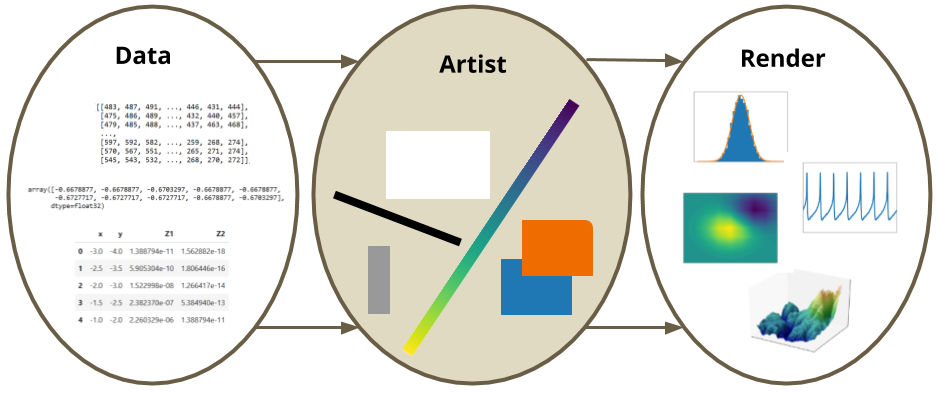
\includegraphics[width=\textwidth]{figures/math/dar.png}
    \caption{Visualization is equivariant maps between data and visual encoding of the variables and assembly of those encodings into a graphic.
    \note{not gonna name these bubbles tau, mu, rho, but might keep the same basic structure of different types of data and encodings }}
    \label{fig:artist_stages}
\end{figure}

\note{should this be in 3rd person passive?}\\
Visualization is generally thought of as structure preserving maps from data into graphics, and in this section we formally define that structure and how it is preserved via equivariant maps. We can then specify that a faithful visual mapping is structure preserving, and apply these constraints to visualizations we may want to develop or implement. We model the data, visual characteristic, and graphic stages of visualization, shown in figure~\ref{fig:artist_stages}, as topological structures that encapsulate types of variables and continuity; by doing so we can develop implementations that keep track of both in ways that let us distribute computation while still allowing assembly and dynamic update of the graphic. 

We introduce a mathematical description of the visualization pipeline where artist $\mathscr{\vartist}$ functions transform data space $\mathscr{\dtotal}$ to an intermediate representation in a prerendered graphic space $\mathscr{\gtotal}$.

\begin{equation}
    \label{eq:artist}
    \mathscr{\vartist}: \mathscr{\dtotal} \rightarrow \mathscr{\gtotal}
\end{equation}

We first describe how we model data(\ref{sec:data}), graphics(\ref{sec:graphic}), and intermediate visual characteristics (\ref{sec:artist}) as fiber bundles. We then discuss the equivariant maps between data and visual characteristics (\ref{sec:artist_nu}) and visual characteristics and graphics (\ref{sec:artist_q}) that make up the artist.

\subsection{Data Space \dtotal}
\label{sec:data}
We build on Butler's proposal of using fiber bundles as a common data representation format for visualization data\cite{butlerVectorBundleClassesForm1992, butlerVisualizationModelBased1989} because fiber bundles are mathematical structures that are flexible enough express all the types of data described in section~\ref{sec:intro_data_structure}.

We model data as the fiber bundle $(\dtotal,\,\dbase,\,\pi ,\,\dfiber)$, where \dtotal\, \dfiber\, and \dbase\ are topological spaces that encode 
\begin{description}
\item[\dfiber] the properties of the variables in the fiber (\ref{sec:data_fiber})
\item[\dbase] the continuity of the records in the base space (\ref{sec:data_base})
\item[\dsection] collections of records (\ref{sec:data_section}). 
\end{description}

and \dtotal\ is the total space of data that \dfiber\ lives in. The bundle is the projection map $\pi$
\begin{equation}
    \label{eq:fiber_bundle}
    \begin{tikzcd}
        \dfiber \arrow[r, hook] & \dtotal \arrow[r, "\pi"] & \dbase
    \end{tikzcd}
\end{equation}

that binds the variables \dfiber\ continuity \dbase. The fiber bundles mentioned in this work are assumed to be trivial\cite{spanier1989algebraic,LocallyTrivialFibre}, unless otherwise specified, because the trivial bundle is $\dtotal=\dbase\times \dfiber$ such that extra structure in the total space \dtotal\ falls out and discussion can be focused on the fiber and base space. 

\subsubsection{Variables: Fiber Space \dfiber}
\label{sec:data_fiber}
The fiber is a topological space that is the set of possible values of the data; the values themselves can be any dimension and type and have any continuity. We use Spivak's description of simplicial database schemas \cite{spivakSIMPLICIALDATABASES} as the basis of our fiber space because he binds the components of the fiber to variable names and types. Spivak constructs a set \ftotal\ that is the disjoint union of all possible objects of types $\{\ftype_0, \ldots, \ftype_n\} \in \ftypes$, where \ftypes\ are the data types of the variables in the dataset. He then defines the single variable set \fttype\ 
\begin{equation}
    \label{eq:data_types}
    \begin{tikzcd}
        \fttype \arrow[r] \arrow[d, "\pi_{\fsection}"'] & \ftotal \arrow[d, "\pi"] \\
        \fnames \arrow[r, "\fsection"']                          & \ftypes       
    \end{tikzcd}
\end{equation}
which is \ftotal\ restricted to objects of type \ftype\ bound to variable name \fname. Given \fsection, the fiber for a one variable dataset is
\begin{equation}
    \dfiber = \ftotal_{\fsection(\fname)} = \ftotal_{\ftype} 
\end{equation}
where \fsection\ is the schema binding variable name \fname\ to its datatype \ftype. A dataset with multiple variables has a fiber that is the cartesian cross product of $\ftotal_{\fsection}$ applied to all the columns:
\begin{equation}
F = \ftotal_{\ftype_1}\times \ldots \ftotal_{\ftype_i} \ldots\times \ftotal_{\ftype_n}
\end{equation}
which is equivalent to 
\begin{equation}
    \dfiber= \dfiber_{0} \times \ldots \times \dfiber_{i}\times\ldots\times \dfiber_{n}
\end{equation}

which allows us to decouple \dfiber\ into components $\dfiber_i$. 

\begin{figure}[H]
    \begin{subfigure}{.5\textwidth}
        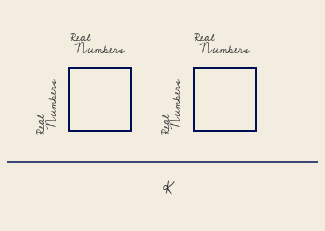
\includegraphics[width=\textwidth]{figures/math/temp_2f.png}
        \caption{}
        \label{fig:fiber_example_plane}
    \end{subfigure}
    \begin{subfigure}{.5\textwidth}
        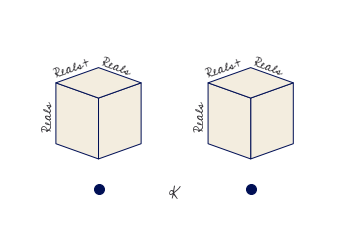
\includegraphics[width=\textwidth]{figures/math/temp_3f.png}
        \caption{}
        \label{fig:fiber_example_cube}
    \end{subfigure}
    \caption{These two datasets have the same base space \dbase\, but figure~\ref{fig:fiber_example_plane} has fiber  $\dfiber=\reals\times\reals$ which is (time, temperature) while figure~\ref{fig:fiber_example_cube} has fiber $\realsp\times\reals^2$ which is (time, wind=(speed, direction))}
    \label{fig:data_fiber_example}
\end{figure}

For example, the data in figure~\ref{fig:fiber_example_plane} is a pair of times and \textdegree C temperature measurements taken at those times. Time is a positive number of type \texttt{datetime} which can be resolved to positive floats $\ftotal_{\texttt{datetime}}= \realsp$. Temperature values are real numbers $\ftotal_{\texttt{float}} = \reals$. The fiber is 
\begin{equation}
    \ftotal =  \realsp \times \reals 
\end{equation} 
where the first component $F_0$ is the set of values specified by $(\fname_0=time,\, \ftype_0=\texttt{datetime},\, \fttype=\mathbb{R}^+)$ and $F_1$ is specified by $(\fname_1=temperature,\, \ftype_1=\texttt{float},\, \fttype=\reals)$. In figure~\ref{fig:fiber_example_cube}, temperature is replaced with wind. This wind variable is of type \texttt{wind} and has two components speed and direction $\{(s,d) \in \reals^{2} \mid  0\leq s,\, 0 \leq d \leq 360\}$ . Therefore, the fiber is 
\begin{equation}
    \dfiber = \realsp \times \reals^{2}
\end{equation} 
such that $F_1$ is specified by $(\fname_1 = wind,\, \ftype_1=\texttt{wind},\, \fttype=\reals^{2})$  

\subsubsection{Measurement Scales: Monoid Actions}
\label{sec:data_monoid}
After specifying \dfiber\, we next describe the ways in which we can transform the values by identifying the monoid actions \monoid\ on the \dfiber. We use monoids as the abstraction because they encode composibilty, which maps well to the data transformation process in a software library \cite{yorgeyMonoidsThemeVariations}. 

A monoid \cite{Monoid2021} $\monoid_i$ is a set with an associative binary operator $\ast:\monoid_i \times \monoid_i\rightarrow \monoid_i$. A monoid has an identity element $e\in \monoid_i$ such that $e\ast a= a \ast e = a$ for all $a \in \monoid_i$. A left monoid action \cite{SemigroupAction2021,ActionNLab} of $\monoid_i$ is a set $\dfiber_i$ with an action $\bullet: \monoid\times \dfiber_i \rightarrow \dfiber_i$ with the properties:
\begin{align*}
    \textbf{associativity}\;& \text{for all } f,g \in \monoid_i \text{ and } x\in \dfiber_i,\, f\bullet(g\bullet x) = (f\ast g) \bullet x\\
    \textbf{identity}\;& \text{for all } x\in \dfiber_i, e\in \monoid_i,\,  e\bullet x = x 
\end{align*}
As with the fiber \dfiber\, the total monoid space \monoid\ is the cartesian product
\begin{equation}
\monoid= \monoid_{0} \times \ldots \times \monoid_{i}\times \ldots \times\ldots \monoid_{n}
\end{equation}
of each monoid $\monoid_{i}$ on $\dfiber_{i}$.  The monoid is also added to the specification of the fiber $(\fname_i,\, \ftype_i,\, \fttype\, \monoid_i)$

Steven's described the measurement scales\cite{stevensTheoryScalesMeasurement1946,leaFormalizationMeasurementScale} in terms of the monoid actions on the measurements: nominal data is permutable, ordinal data is monotonic, interval data is translatable, and ratio data is scalable \cite{weissteinSimilarityTransformation}. For example, given  the fiber $(\fname=temperature,\, \ftype=\texttt{float},\,\fttype=\reals)$ which is interval data:
\begin{itemize}
    \item monoid operator addition $\ast = +$
    \item monoid operations: $f: x\mapsto x + 1 $, $g: x\mapsto x + 2  $
    \item monoid action operator composition $\bullet = \circ$
\end{itemize}
then the translation monoid actions on temperature satisfy the condition
\begin{equation}
    \begin{tikzcd}
        \reals \arrow[rd, "(x+ 1\degree)\circ(x+2\degree)"] \arrow[d, "x+ 1\degree"'] &            \\
        \reals \arrow[r, "x+ 2\degree"']                                   & \reals
    \end{tikzcd}
\end{equation}
where $1\degree$ and $2\degree$ are valid distances between two temperatures $x$.  


\subsubsection{Continuity: Base Space $K$} 
\label{sec:data_base}
The advantage of fiber bundles is they provide a way to encode the continuity in a dataset as the base space \dbase\ without making assumptions as to what that continuity is. In turn this representation of continuity can then be used to keep track of how the data fits together, for example if a visualization of a very large dataset calls for parallelization.  

\begin{figure}[H]
    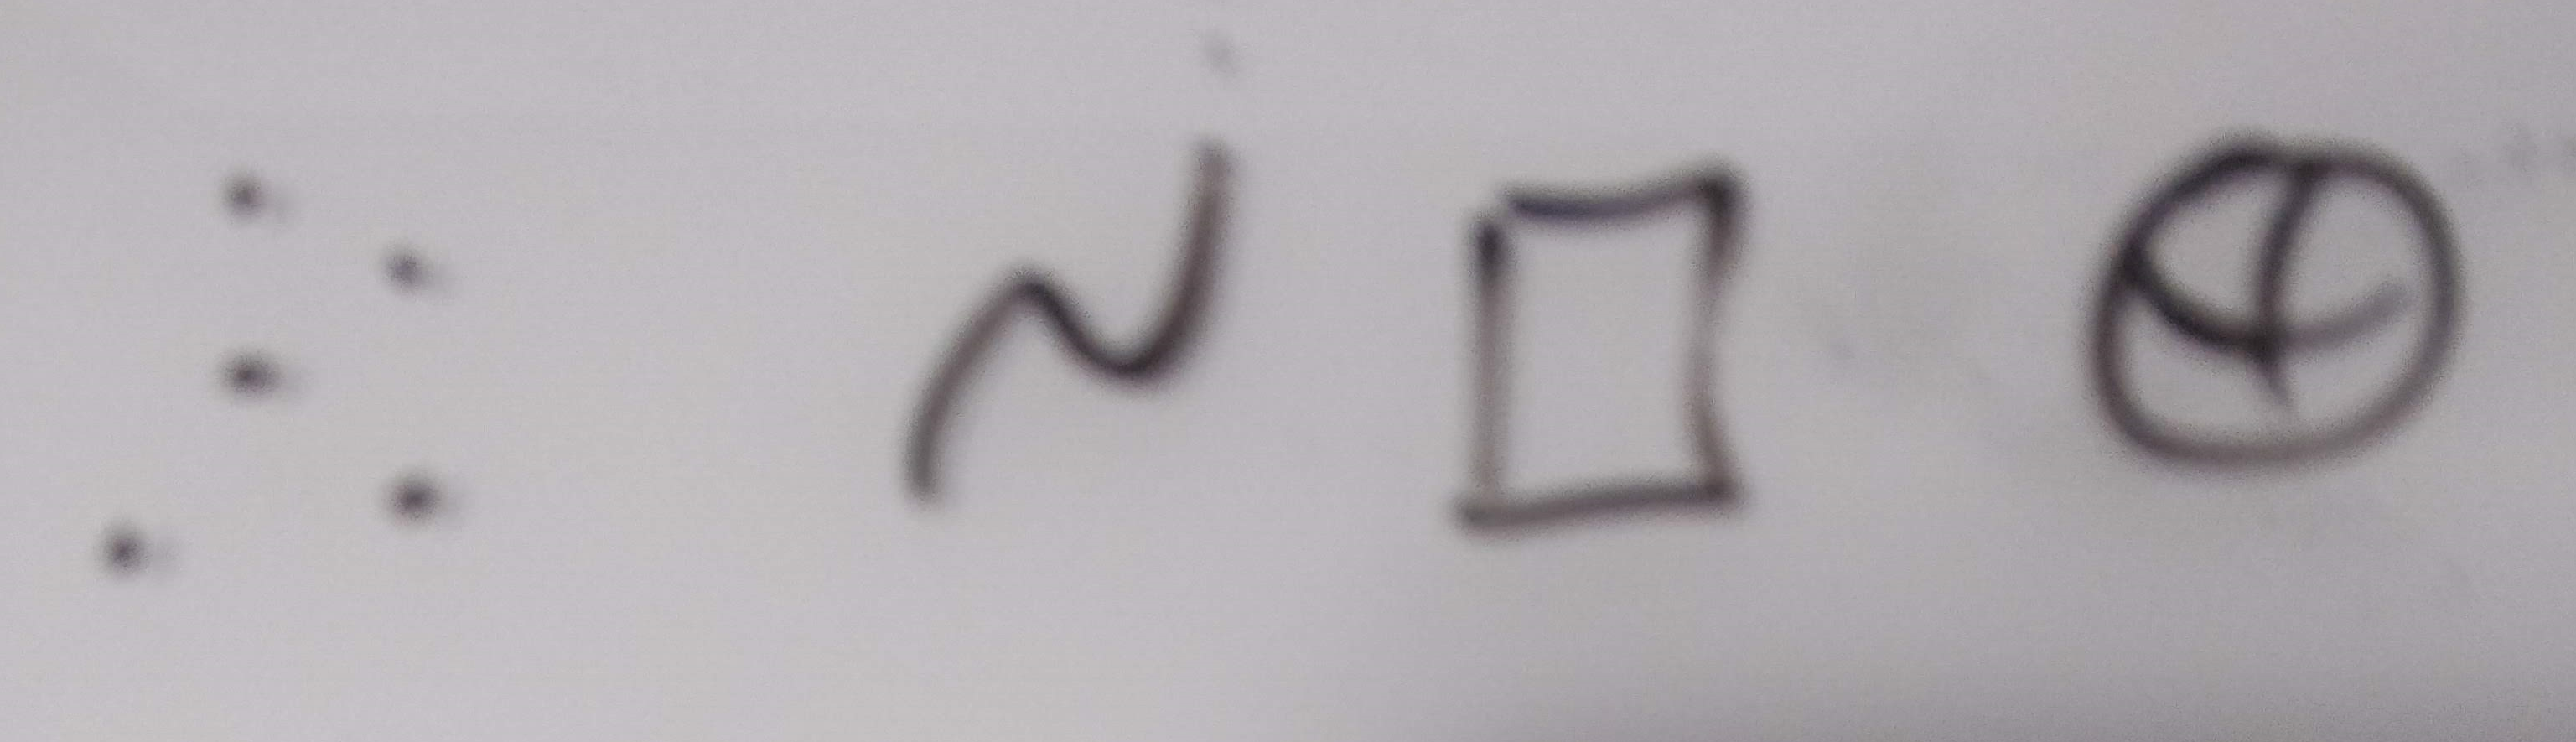
\includegraphics[width=.5\textwidth]{figures/math/k_different_types.png}
    \caption{The topological base space \dbase\ encodes the connectivity of the data space, for example if the data is independent points or a map or on a sphere}
    \label{fig:base_space_types}
\end{figure}
As illustrated in figure~\ref{fig:base_space_types}, \dbase\ is akin to an indexing space into \dtotal\ that describes the structure of \dtotal.  \dbase\ can have any number of dimensions and can be continuous or discrete. 

\begin{figure}[H]
    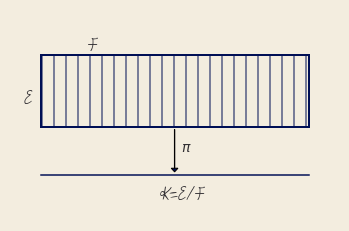
\includegraphics[width=.5\linewidth]{figures/math/k_qspace.png}
    \caption{The base space \dtotal\ is divided into fiber segments \dfiber. The base space \dbase\ acts as an index into the records in the fibers.
    \note{this figure might be good all the way up top to lay out the components of fb}}
    \label{fig:base_space_div}
\end{figure}

Formally \dbase\ is the quotient space \cite{QuotientSpaceTopology2020} of \dtotal\, meaning it is the finest space\cite{aurouxMath131Introduction} such that every $\dbasepoint \in \dbase$ has a corresponding fiber $\dfiber_k$\cite{QuotientSpaceTopology2020}. In figure~\ref{fig:base_space_div}, \dtotal\ is a rectangle divided by vertical fibers \dfiber, so the minimal \dbase\ for which there is always a mapping $\pi: \dtotal\rightarrow \dbase$ is the line. 

As with fibers and monoids, we can decompose the total space into components $\pi:\dtotal_i\rightarrow \dbase$ where
\begin{equation}
    \pi:\dtotal_1\oplus\ldots\oplus \dtotal_i \oplus\ldots \oplus \dtotal_n \rightarrow \dbase
\end{equation}

which is a decomposition of \dfiber. The \dbase\ remains the same because the connectivity of records does not change just because there are fewer elements in each record.

\begin{figure}[ht!]
    \begin{subfigure}{.5\textwidth}
        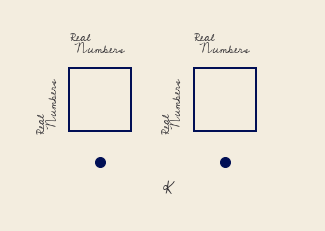
\includegraphics[width=\textwidth]{figures/math/temp_1k.png}
        %% add box around neighboring P and Map
        \caption{}
        \label{fig:base_example_discrete}
    \end{subfigure}
    \begin{subfigure}{.5\textwidth}
        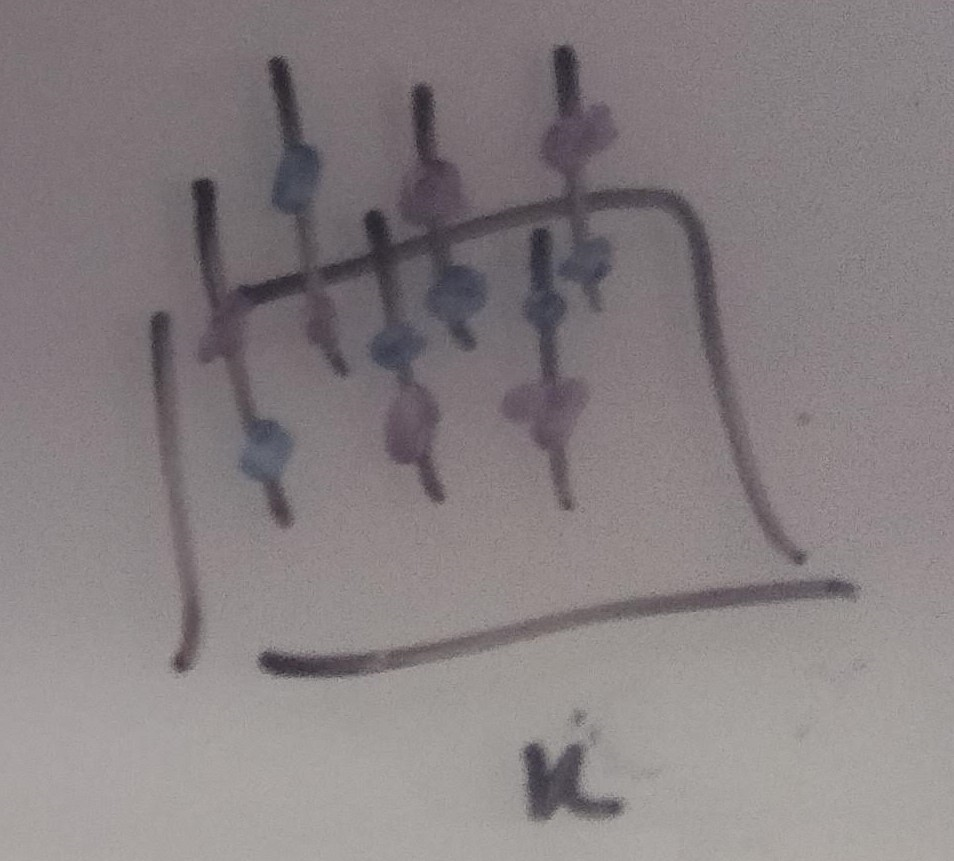
\includegraphics[width=\textwidth]{figures/math/temp_2k.png}
        \caption{}
        \label{fig:base_example_continuous}
    \end{subfigure}
    \caption{These two datasets have the same (time, temperature) fiber. In figure~\ref{fig:base_example_line} the total space \dtotal\ is discrete over points $\dbasepoint \in \dbase$, meaning the records in the fiber are also discrete. In figure~\ref{fig:base_example_plane} \dtotal\ lies over the continuous interval \dbase, meaning the records in the fiber are sampled from a continuous space. 
    \note{revamp figure: F=Plane, k1 = dots, k2=line}}
    \label{fig:base_example}
\end{figure}

The datasets in figure~\ref{fig:base_example} have the same fiber of (temperature, time). In figure~\ref{fig:base_example_discrete} the fibers lie over discrete \dbase\ such that the records in the datasets in the fiber bundles are discrete. The same fiber in figure~\ref{fig:base_example_continuous} lies over a continuous interval \dbase such that the records are samples from a continuous function defined on \dbase.

\subsubsection{Data: Sections \dsection}
\label{sec:data_section}
While the fiber and base space describe the general structure of all data that lives in the fiber bundle, the sections $\dsection: \dbase\rightarrow \dtotal$ define the datasets that live in the fiber. We generalize Spivak's description of the section as a table of records \cite{spivakSIMPLICIALDATABASES} to any sort of structured dataset such that 
\begin{equation}
    \begin{tikzcd}
        \dfiber \arrow[r, hook] & \dtotal \arrow[d, "\pi"'] \\
                          & \dbase \arrow[u, "\dsection"', bend right]
    \end{tikzcd}
\end{equation}
such that there is always a map $\pi(\dsection(\dbasepoint)) = \dbasepoint$. There can be many sections \dsection; the space of global sections is $\Gamma(\dtotal)$. For a trivial fiber bundle, the section is 
\begin{equation}
    \label{eq:section_return}
    \dsection(\dbasepoint) = (\dbasepoint, (g_{\dfiber_{0}}(\dbasepoint), \ldots, g_{\dfiber_{n}}(\dbasepoint)))
\end{equation}
where $g: \dbase \rightarrow \dfiber$ is the index function into the fiber. Because we can decompose the bundle and the fiber, we can formulate $\dsection$ as 
\begin{align}
\dsection= (\dsection_0,\ldots, \dsection_i, \dots, \dsection_n) 
\end{align}
where each section $\dsection_i$ is a variable or set of variables. 

\begin{figure}[H]
    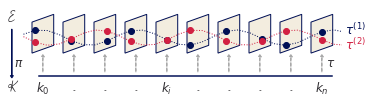
\includegraphics[width=.5\linewidth]{figures/math/fiberbundle.png}
    \caption{ Fiber (time, temperature) with an interval \dbase\ basespace. The sections $\dsection_i$ and $\dsection_j$ are constrained such that the time variable must be monotonic, which means each section is a timeseries of temperature values. They are included in the global set of sections  $\dsection_1, \dsection_2 \in \Gamma(\dtotal)$}
    \label{fig:data_sections}
\end{figure}

In the example in figure~\ref{fig:data_sections}, the fiber is $(time, \, temperature)$ as described in figure~\ref{fig:data_fiber_example} and the base space is the interval \dbase. The section $\dsection_i$ resolves to a series of monotonically increasing in time records of (time, temperature) values. Section $\dsection_j$ returns a different timeseries of (time, temperature) values. Both sections are included in the global set of sections $\dsection_1, \dsection_2 \in \Gamma(\dtotal)$.

\subsubsection{Sheaf and Stalk}
\label{sec:data_sheaf_stalk}
Often a graphic may need to be updated with live data or support zooming in on a segement of the dataset; to support working with a subset of data, we can use the sheaf $\mathcal{O}(\dtotal)$. All fiber bundles are locally trivial, which means that \dtotal\ restricted over a small enough neighborhood $U \subset \dbase$ is a locally trivial bundle over $U$\cite{LocallyTrivialFibre}. The sheaf $O(\dtotal)$ is the localized section of fibers $\iota^*\dsection: U \rightarrow \iota^*\dtotal$

\begin{equation}
    \label{eq:sheaf}
    \begin{tikzcd}
        \iota^*\dtotal \arrow[d, "\pi"']           & \dtotal \arrow[d, "\pi"'] \arrow[l, "\iota^*"']         \\
        U \arrow[u, "\iota^*\dsection"', bend right] & \dbase \arrow[u, "\dsection"', bend right] \arrow[l, "\iota"']
    \end{tikzcd}
\end{equation}
pulled back over the neighborhood $U$ via the inclusion map $\iota: U \rightarrow \dbase$. The localized section is the germ $\xi^*\dsection$. The neighborhood of points $\dbasepoint_i$ surrounding the point \dbasepoint\ the sheaf lies over is the stalk $\mathcal{F}_b$ \cite{StalkSheaf2019,spanier1989algebraic}. While \dtotal\ is only the fiber $\dfiber_k$ over a specific \dbasepoint, the stalk includes nearby records because the sheaf lies over the neighborhood $U$. While this can be useful for visual transforms, often the extra needed information can be found in the smaller jet bundle $\mathcal{J}$ \cite{JetBundle2020,musilovaCalculusVariationsJet2016}. For example, line thickness requires the derivative of the given position to be rendered, which can be found in $\dtotal^\prime=\dtotal+\mathcal{J}(\dtotal)$


\subsection{Graphic: \gtotal}
\label{sec:graphic}  
We can separate the structure of the graphic from the properties of the output format by modeling the space of graphics as a fiber bundle  $(\gtotal, \gbase, \pi, \gfiber)$. As with data, the fiber bundle is for a class of graphics with shared base space \gbase (~\ref{sec:graphic_fiber}) and fiber \gfiber (~\ref{sec:graphic_base}) and the sections \gsection (~\ref{sec:graphic_section}) encode a graphic where the visual characteristics are fully specified.

\subsubsection{Idealized Display \gfiber}
\label{sec:graphic_fiber}
The fiber \gfiber\ is an idealized infinite resolution version of the target display space, for example a 2D screen or 3D printer. In this work, we assume a 2D opaque image $\dfiber=\reals^5$ with elements 
\begin{equation}
(x,\, y,\, r,\, g,\, b) \in \gfiber
\end{equation}
such that a rendered graphic only consists of 2D position and color. To support overplotting and transparency, the fiber could be $\dfiber=\reals^{7}$ such that $(x, y, z, r, g, b, a) \in \gfiber$ specifies the target display. The location coordinates $x$ and $y$ are defined in terms of the display, while the $(r,g,b)$ values are filled in via a lookup on \gbase. 

\subsubsection{Continuity of the Graphic \gbase} 
\label{sec:graphic_base}
An assumption of graphical representations is that they match the continuity of the data\cite{tufteVisualDisplayQuantitative2001,friendlyBriefHistoryData2008}, but the underlying topology \gbase\ of a graphic may need more dimensions than the data topology \dbase\ so that the glyph can be defined in \dfiber. Therefore we define the base space mapping from graphic \gbase to data \dbase 
\begin{equation}
    \begin{tikzcd}
        \dtotal \arrow[d, "\pi"'] & \gtotal \arrow[d, "\pi"'] \\
        \dbase                   & \gbase \arrow[l, "\vindex"']
        \end{tikzcd}
\end{equation}

 as the deformation retraction \cite{RetractionTopology2020} $\vindex: \gbase \rightarrow \dbase$ that goes from a region $\gbasepoint \in \gbase_{\dbasepoint}$ to its associated point $\gbasepoint$, such that when $\vindex(\gbasepoint) = \dbasepoint$,\, $\vindex^*\dsection(\gbasepoint) = \dsection(\gbasepoint)$. While dimensions can be added to \gbase, it retains the same continuity as \dbase.
 
\begin{figure}
    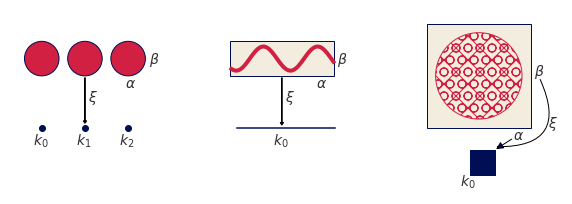
\includegraphics[width=1\textwidth]{figures/math/retraction_maps.png}
    \caption{The scatter and line graphic base spaces have one more dimension of continuity than \dbase\ so that \gbase\ can encode physical aspects of the glyph, such as shape (a circle) or thickness. The heatmap has the same continuity in the graphic \gbase\ as in the data \dbase. \note{add $\alpha, \beta$ coordinates to figures}}
    \label{fig:graphic_retraction_map}
\end{figure}

In figure~\ref{fig:graphic_retraction_map} each disk $\gbase_{\dbasepoint}$ indexes how elements in \gfiber\ are glued together to generate a single glyph that is the visual representation of a single record in $\dfiber_{\dbasepoint}$. For the line, the region \gy\ over a point $\gx_i$ specifies the thickness of the line in \gbase\ for the corresponding \dsection\ on \dbase. The heatmap has the same continuity in data space and graphic space such that no extra dimensions are needed. 

 
\subsubsection{Renderable Glyph \gsection}
\label{sec:graphic_section}
%pick a pixel which is the bounding box
A section $\gsection: \gbase\rightarrow \gtotal$ defines a piece of the graphical representation of the data. Evaluated on a single \gbasepoint\, \gsection\ returns a single element in \gfiber\. For a 2D screen, the pixel is defined as a region $p=\left[y_{top}, y_{bottom}, x_{right}, x_{left}\right]$ of the rendered graphic. Since the x and y in $p$ are in the same coordinate system as the x and y components of \gfiber\,  the inverse map of the bounding box $\gbase_{p} ={\gsection_{xy}}^{-1}(p)$ is a region $\gbase_p \subset \gbase$. Integrating over this region on \gbase\
\begin{align}
    r_p &= \iint\limits_{S_p} \rho_r(s)ds^{2}\\
    g_p &= \iint\limits_{S_p} \rho_g(s)ds^{2}\\
    b_p &= \iint\limits_{S_p} \rho_b(s)ds^{2}
\end{align}
yields the color of the pixel $p$.

\begin{figure}
    \includegraphics[width=\textwidth]{figures/math/graphic_render.png}
    \caption{To render a graphic, a pixel $p$ is selected in the display space, which is defined in the same coordinates as the x and y components in \gfiber\.  The inverse mapping ${\gsection_{xy}}^(p)$ returns a region $\gbase_{p} \subset \gbase$. $\gsection(\gbase_{p})$ returns the list of elements $(x,\,y,\,r,\,g,\,b) \in \gfiber$ that lie over $\gbase_{p}$. The integral over the $(r,\,g,\,b)$ elements is the color of the pixel.}
    \label{fig:graphic_rho_lookup}
\end{figure}
As shown in figure~\ref{fig:graphic_rho_lookup}, the output space queries into the graphic bundle to render the image. We select a pixel $p$ in the output space, inverse map the region of the pixel into $\gbase_p \subset \gbase$, then compute the section $gsection$ over the region $\gbase_p$. The section yields the set of elements in \gfiber\ that specify the $(r, g, b)$ values corresponding to the region $p$. The color of the pixel is then obtained by taking the integral of $\gsection_{rgb}(\gbase_p)$. 

\subsection{Artist}
\label{sec:artist}
The artist is the function that converts data into graphics; its name is taken from the analogous part of Matplotlib\cite{hunterArchitectureOpenSource} that builds visual elements to pass off to the renderer. The artist \vartist\ is a mapping from \dtotal\ padded with data from $\mathcal{J}(\dtotal)$ to a graphic that is a section \gsection\ in  $\Gamma(\gtotal)$
\begin{equation}
    \label{eq:artist_diagram}
    \begin{tikzcd}
        \dtotal^{\prime} \arrow[r, "\vchannel"] \arrow[rd, "\pi"'] & \vtotal \arrow[d, "\pi"] & \vindex^*\vtotal \arrow[r, "\vmark"] \arrow[d, "\vindex^*\pi"'] \arrow[l, "\vindex^*"'] & \Gamma(\gtotal) \arrow[ld, "\pi"] \\
                                              & \dbase                  & \gbase \arrow[l, "\vindex"']                                              &                    
        \end{tikzcd}
\end{equation}
with an intermediate fiber bundle \vtotal\ to hold visual representations and stages
\begin{enumerate}
    \item \vindex\ binding the continuity in the graphic to the continuity in the data (~\ref{sec:graphic_base})
    \item \vchannel\ conversion of data into visual characteristics (~\ref{sec:artist_nu})
    \item \vmark\ assembly of visual variables into a glyph (~\ref{sec:artist_q})
\end{enumerate}
 
of the visual transformation illustrated in figure~\ref{fig:artist_stages}. The functions \vindex\, \vchannel\ and \vmark\ are defined such that they can be evaluated on a single section \dsection, which allows the artist to be implemented such that it does not need all the data. This allows for artists tuned to distributed and streaming data. 

\subsubsection {Visual Fiber Bundle \vtotal}
The visual fiber bundle (\vtotal, \dbase, $\pi$, \vfiber) has section $\vsection: \vtotal \rightarrow \dbase$ that resolves to a visual variable \cite{bertinIIPropertiesGraphic2011,munznerMarksChannels} in fiber \vfiber. The fiber space \vfiber\ is defined in terms of the parameters of the visualization specification- for example aesthetics  in ggplot \cite{wickhamGgplot2ElegantGraphics2016a}, channels in vega\cite{satyanarayanDeclarativeInteractionDesign2014} or parameters in VTK\cite{hanwellVisualizationToolkitVTK2015} and Matplotlib.

\begin{table}[H]
    \renewcommand{\arraystretch}{2}
    \begin{tabulary}{\textwidth}{|l|L|l|}\hline
     $\bm{\vchannel_{i}}$                      & $\bm{\vsection_{i}}$                                                            & $\bm{codomain(\vchannel_{i})}$  \\ \hline                                              
    position                    & x, y, z, theta, r                                                          & $\mathbb{R}$   \\ \hline
    size                        & linewidth, markersize                                            & $\mathbb{R}^{+}$   \\ \hline
    shape                       & markerstyle                                                      & $\{f_{0}, \ldots, f_{n}\}$ \\ \hline
    color                       & color, facecolor, markerfacecolor, edgecolor  & $\mathbb{R}^{4}$ \\ \hline
    \multirow{2}{*}{texture}    & hatch                                                            & $\mathbb{N}^{10}$\\\cline{2-3}
                                & linestyle                                                        & $\{f_{0}, \ldots, f_{n}\} \times (\mathbb{R}, \mathbb{R^+}^{n, n\%2=0})$ \\ \hline              
    \end{tabulary}
    \caption{Some possible components of the fiber \vfiber\ for a visualization function implemented in Matplotlib}
    \label{tab:mpl_visual_variable_fiber}
\end{table}

Table~\ref{tab:mpl_visual_variable_fiber} is a sample of the fiber space for Matplotlib \cite{hunterMatplotlib2DGraphics2007}. A section \vsection is a tuple of visual values that specifies the visual characteristics of a part of the graphic. For example, given a fiber of $\{xpos, ypos, color\}$ one possible section could be  $\{.5, .5, (255, 20,147)\}$. The $codomain(\vchannel_i)$ determines the monoid actions on $\vsection_i$. These fiber components are implicit in the library, by making them explicit as components of the fiber we can build consistent definitions and expectations of how these parameters behave. 

\subsubsection{Visual Channels}
\label{sec:artist_nu}
\begin{figure}
    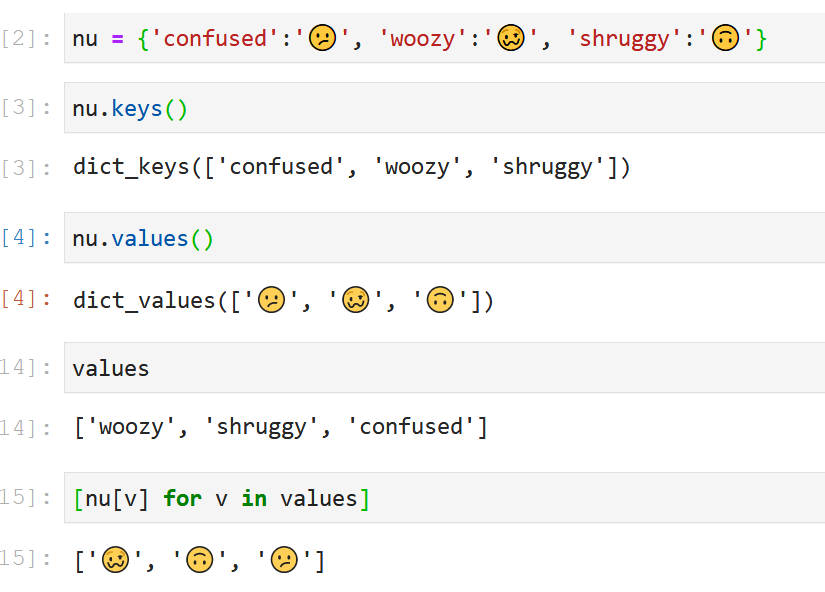
\includegraphics[width=\textwidth]{figures/math/equivariance_nu.png}
    \caption{In this artis, \vchannel\ maps the strings to the emojis. For \vchannel\ to be equivariant, a shuffle in the words should have an equivalent shuffle in the emojies, and a shuffle in the emojies should have an equivalent shuffle in the words.}
    \label{fig:artist_nu}
\end{figure}
As introduced in section~\ref{sec:intro_visual_variables}, there are many ways to encode data visually. We define the visual transformers \vchannel\ as the set of independent conversion functions 
\begin{equation}
    \label{eq:nu_expanded}
    \{\vchannel_{0}, \ldots, \vchannel_{n}\}: \{\dsection_{0}, \ldots, \dsection_{n}\} \mapsto \{\vsection_{0}, \ldots, \vsection_{n}\}
\end{equation}
where $\vchannel_i: \dsection_i \mapsto \vsection_i$ is an equivariant map such that there is a monoid homomorphism from $\dfiber_{i}$ to $vfiber_{i}$. A validly constructed \vchannel\ is one where the  diagram of the monoid transform $m$
\begin{equation}
    \label{eq:nu_categorical}
\begin{tikzcd}
    \dtotal_i \arrow[r] \arrow[r, "\vchannel_i"] \arrow[d, "m_{\delement}"'] & \vtotal_i \arrow[d, "m_{\velement}"] \\
    \dtotal_i \arrow[r, "\vchannel_i"]                           & \vtotal_i               
\end{tikzcd}
\end{equation}
commutes such that $\vchannel_i(m_{\delement}(\dtotal_i)) = m_{\velement}(\vchannel_i(\dtotal_i))$. This equivariance constraint yields guidance on what makes for an invalid transform. For example, the conversion $\vchannel_{i}(x) = .5$ does not commute under translation monoid action $t(x) = x+2$  
\begin{align}
    \vchannel(t(\delement + 2)) & \overset{?}{=} \vchannel(\delement) + \vchannel(2)\\
    .5 &\neq .5 + .5
\end{align}

On the other hand figure~\ref{fig:artist_nu} illustrates a valid \vchannel\ mapping from \textbf{Strings} to symbols. The group action on these sets is permutation, so shuffling the words must have an equivalent shuffle of the symbols they are mapped to. To preserve ordinal and partial order monoid actions, \vchannel\ must be a monotonic function such that given $\delement_1, \delement_2 \in \dtotal_{i}$, $\text{ if } delement_1 \leq delement_2 \text{ then } \vchannel (\delement_1) \leq \vchannel(\delement_2)$. For interval scale data, \vchannel\ is equivariant under translation monoid actions if $\vchannel (x + c) = \vchannel(x) + \vchannel(c)$. For ratio data, there must be equivalent scaling $ \vchannel(xc) = \vchannel(x)\vchannel(c)$.

\subsubsection{Assembling Marks}
\label{sec:artist_q}
\begin{figure}[H]
    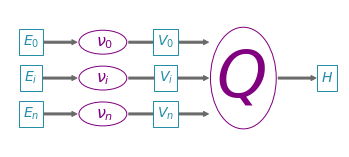
\includegraphics[width=\textwidth]{figures/math/path_of_q}
    \caption{\vchannel\ functions convert data $\dsection_i$ to visual characteristics $\vsection_i$, then \vmark\ assembles $\vsection_i$ into a graphic $\gsection$ such that there is a map \vindex\ preserving the continuity of the data. \gsection\ applied to a region of connected components $\gbase_{\dbasepathpoint}$  generates a graphical mark.} 
    \label{fig:artist_q}
\end{figure}

As shown in figure~\ref{fig:artist_q}, the assembly function \vmark\ combines the fiber $\dfiber_i$ wise \vchannel\ transforms into a single glyph. Together, \vchannel\ and \vmark\ are a map-reduce operation: map the data into their visual encodings, reduce the encodings into a glyph. As with \vchannel\, the constraint on \vmark\ is that for every monoid actions on the input \vsection\ there is a corresponding monoid action on the output \gsection. 

Since we define the equivariant map as  $\vmark: \vsection \mapsto \gsection$, we define an action on the subset of graphics $\vmark(\Gamma(\vtotal)) \in \Gamma(\gtotal)$ that \vmark\ can generate. We then define the constraint on \vmark such that if \vmark\ is applied to $\vsection, \vsection^{\prime}$ that generate the same \gsection\, then the output of both sections acted on by the same monoid $m$ must be the same.   

Lets call the visual encodings $\Gamma(\vtotal)=X$ and the graphic $\vmark(\Gamma(\vtotal))=Y$. If for all monoids $m \in \monoid$ and for all $\vsection, \vsection^{\prime} \in X$, the output is equivalent 
\begin{equation}
\vmark(\vsection) = \vmark(\vsection^{\prime})\implies \vmark(m\circ\vsection) = \vmark(m\circ\vsection^{\prime})
\end{equation}
then a group action on $Y$ can be defined as $m\circ \gsection = \gsection^{\prime}$. The transformed graphic $\gsection^{\prime}$ is equivariant to a transform on the visual bundle $\gsection^{\prime}=\vmark(m\circ \vsection)$ on a section that $\vsection \in \vmark^{-1}(\gsection)$ that must be part of generating \gsection. 



\begin{figure}[H]
    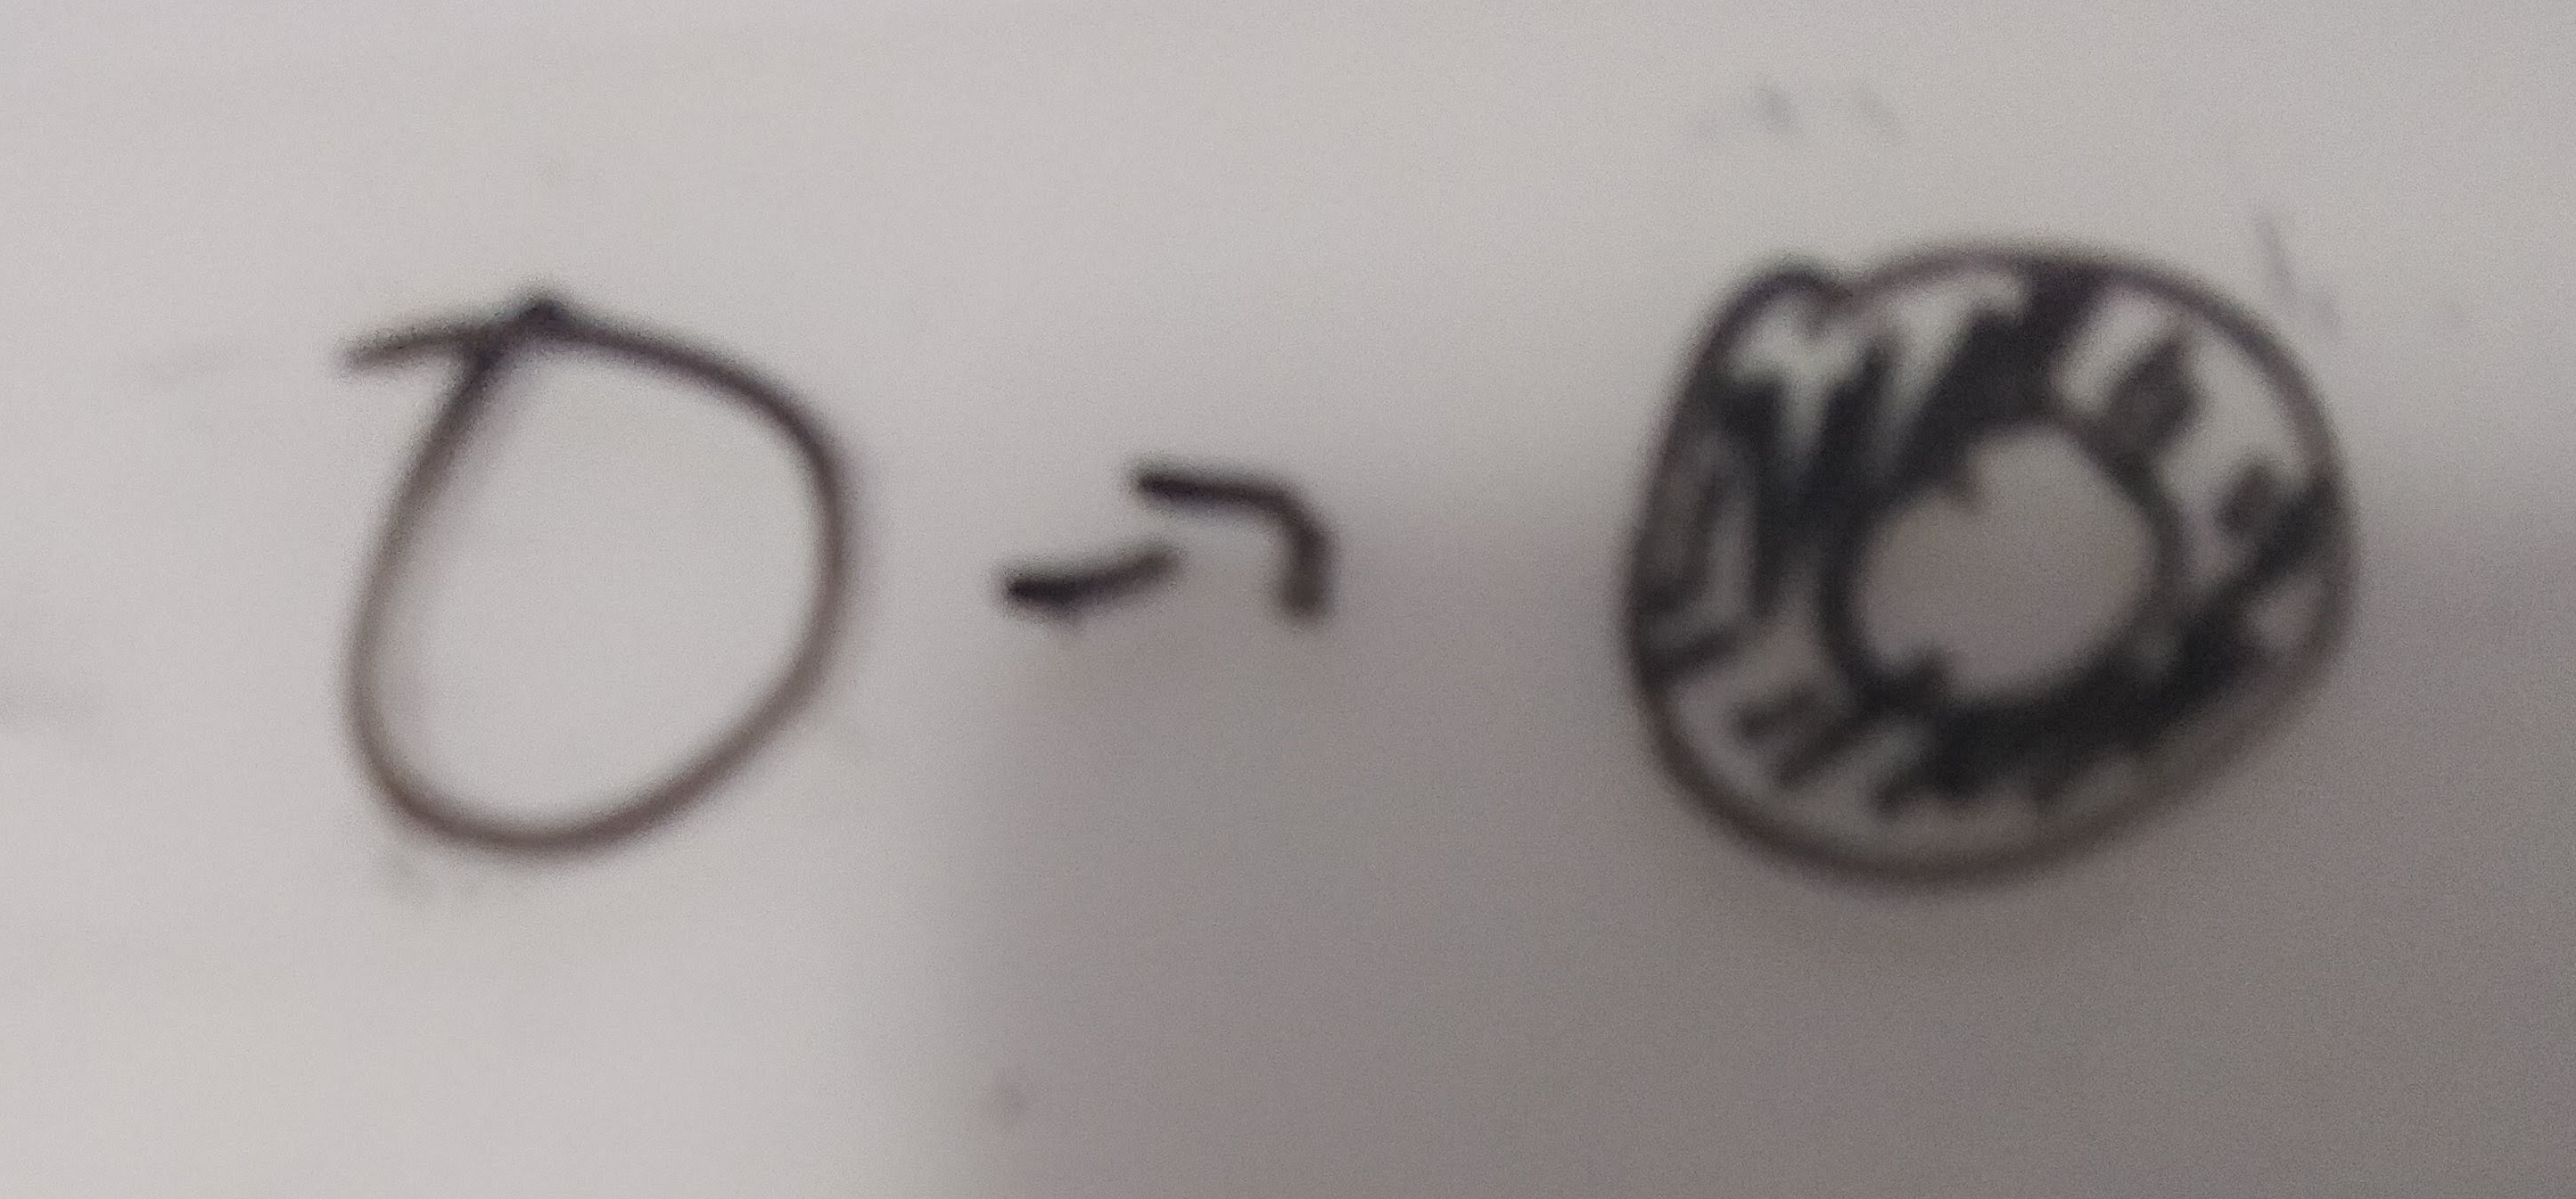
\includegraphics[width=\textwidth]{figures/math/diff_type_q.png}
    \caption{These two glyphs are generated by the same \vmark\ function, but differ in the value of the edge thickness parameter $\vsection_i$. A valid \vmark\ is one where a shift in $\vsection_i$ is reflected in the glyph generated by \gsection.}
    \label{fig:artist_mark_change}
\end{figure}

The glyph in figure~\ref{fig:artist_mark_change} has the following characterstics \vfiber specified by  $(xpos,\, ypos,\, color,\, thickness)$ such that one section is $\vsection=(0,0,0,1)$ and $\vmark(\vsection) = \gsection$ generates a piece of the thin hollow circle. The equivariance constraint on \vmark is that the action $m=(e, e, e, x+2)$, where e is identity, applied to \vsection\ such that $\vsection^{\prime}=(e,e,e,3)$ has an equivalent action on \gsection that causes $\vmark(\vsection^{\prime})$ to be equivalent to the thicker circle in figure~\ref{fig:artist_mark_change}.

\note{DEGENERATE Q - drawing a blank if this is necessry and if so how\\
Check a well defined map $\monoid\times Y \rightarrow Y$}

To output a mark  \cite{bertinIIPropertiesGraphic2011,carpendaleVisualRepresentationSemiology}, \vmark\ is called with all the regions \gbasepoint\ that map back to a set of connected components $\dbasepath \subset \dbase$:
\begin{equation}
\dbasepath = \{\dbasepathpoint \in \dbase \text{ s. t. } \exists \gamma \text{ s.t. } \gamma(0)=\dbasepoint \text{ and }\gamma(1)=\dbasepathpoint\}
\end{equation}
where the path\cite{ConnectedSpace2020}  $\gamma$ from \dbasepoint\ to \dbasepathpoint\ is a continuous function from the interval [0,1]. We define the mark as the graphic generated by $\vmark(\gbase_{\dbasepathpoint})$

\begin{equation}
    \begin{tikzcd}
        \gtotal \arrow[r, shift left] & \gbase_\dbasepathpoint \arrow[rr, "\vindex(\gbasepoint)", shift left] \arrow[l, "\gsection(\gbase_\dbasepathpoint)"] &  & \dbasepath_{\dbasepoint} \arrow[ll, "\vindex^{-1}(\dbasepath)"]
        \end{tikzcd}
    \label{eq:mark}
\end{equation}
such that for every mark there is at least one corresponding section on \dbase.

\subsubsection{Sample Qs}
%rewrite as alpha/beta 
In this section we formulate the minimal Q that will generate distinguishable graphical marks: non-overlapping scatter points, a non-infinitely thin line, and a heatmap. 
\label{sec:artist_example_scatter}
\begin{figure}[H]
    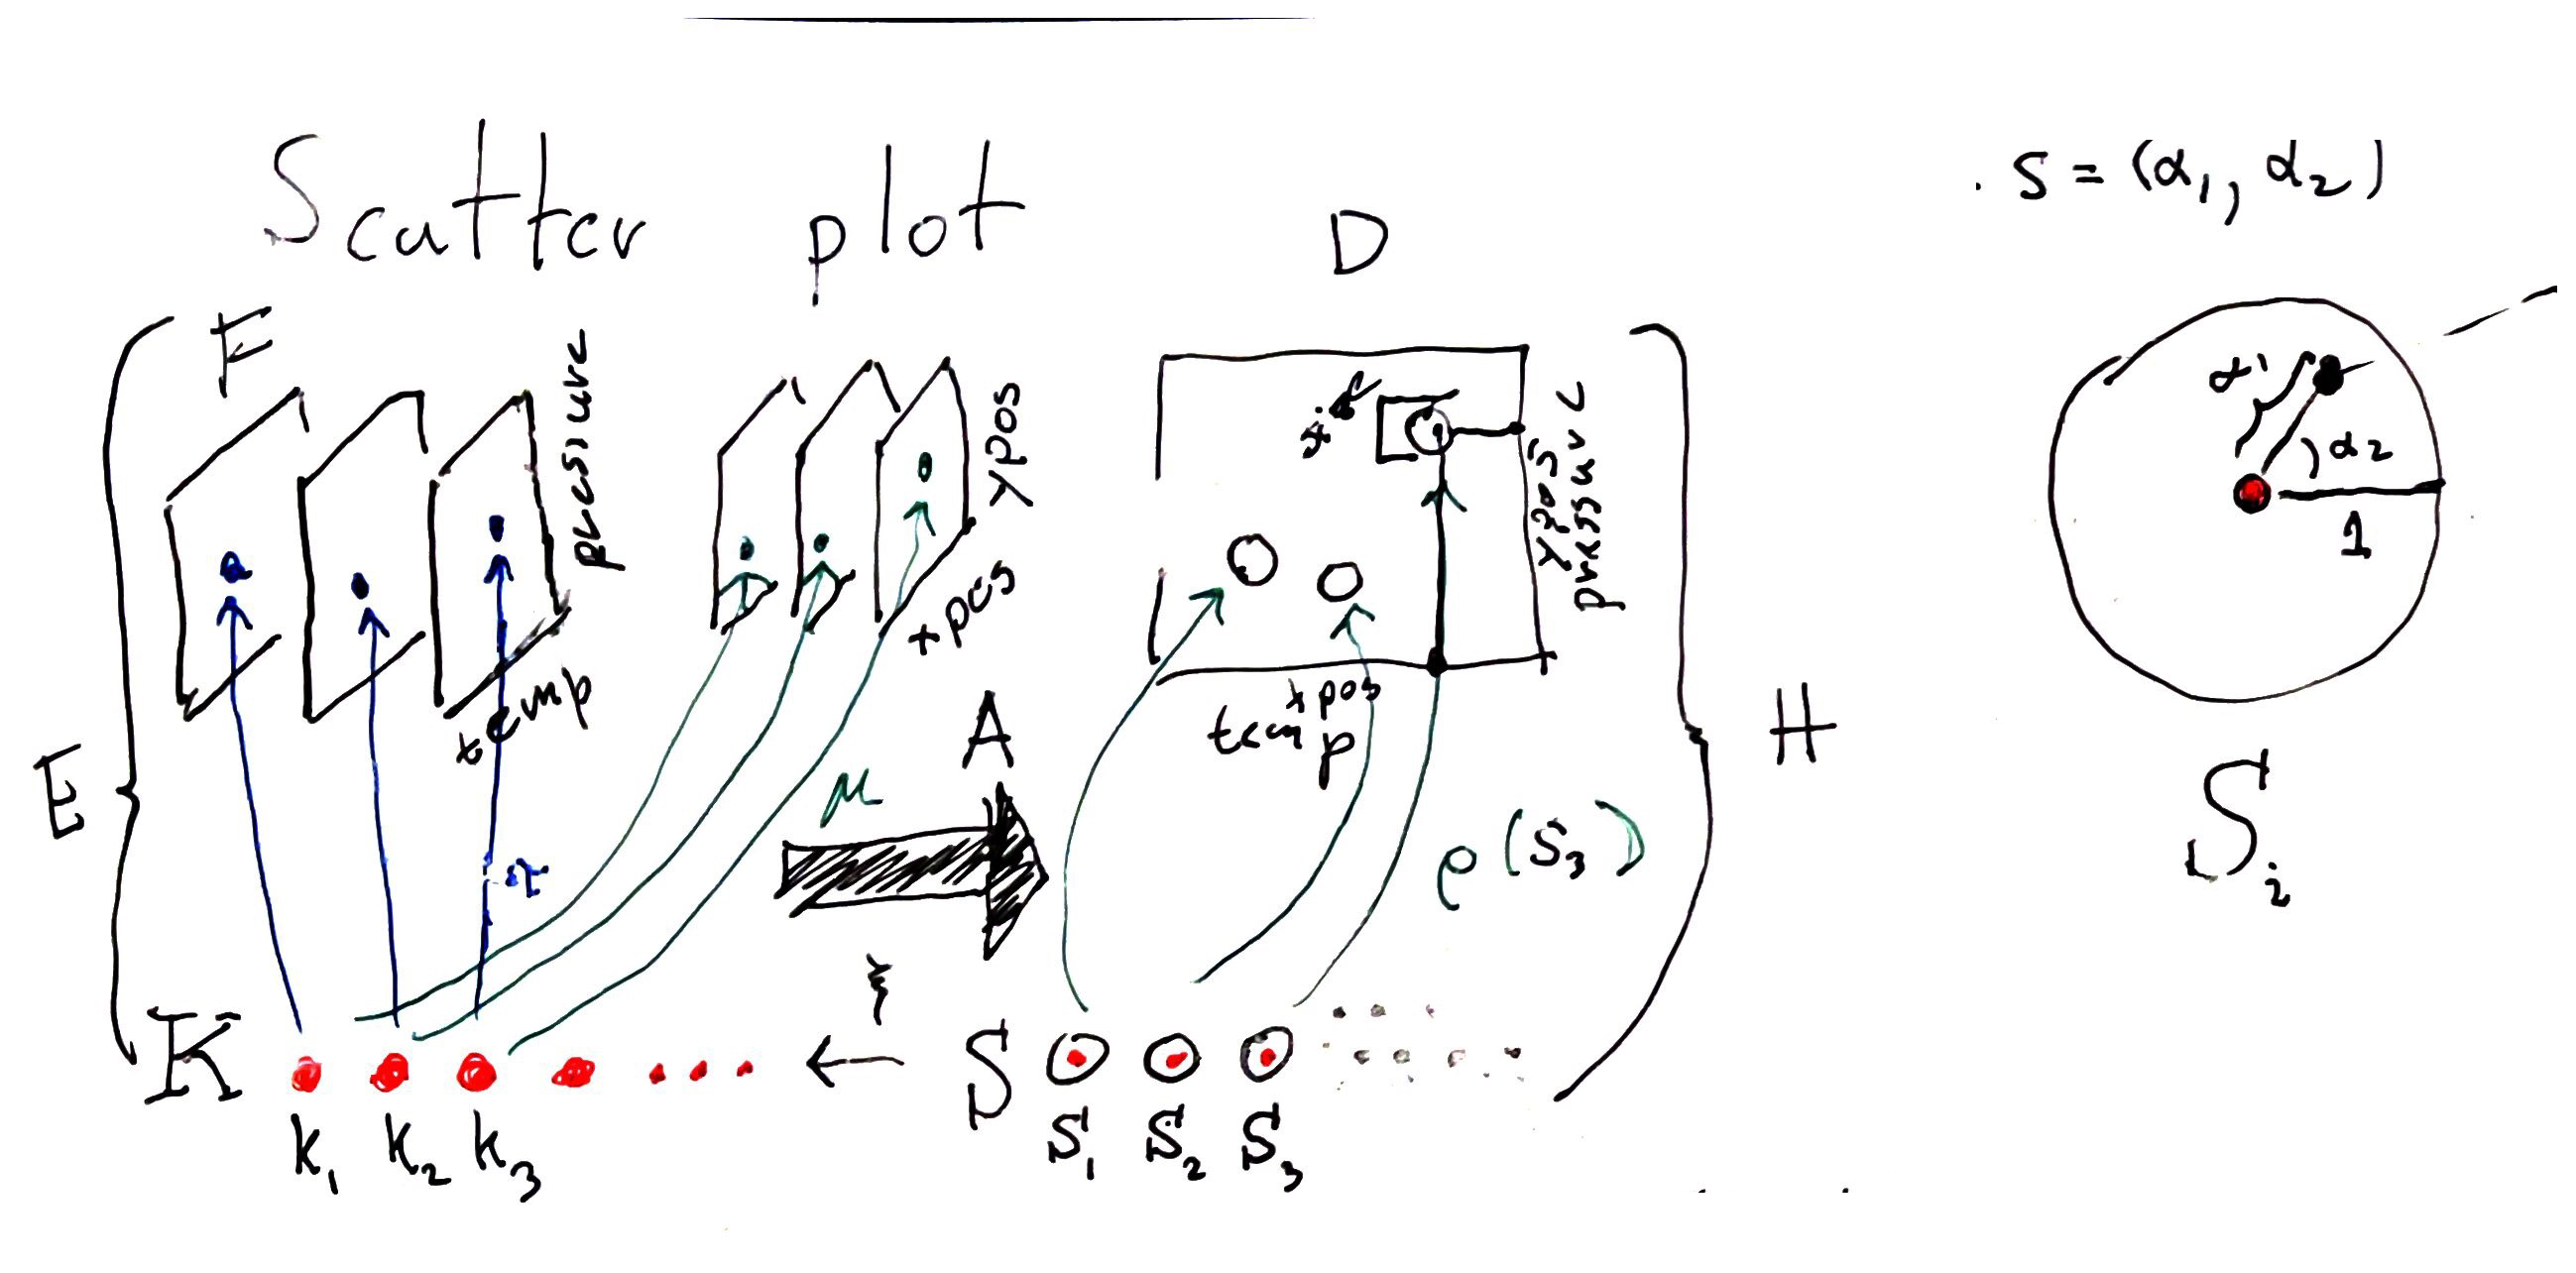
\includegraphics[width=\textwidth]{figures/math/scatter.png}
    \caption{The data is discrete points (temperature, time). Via \vchannel\ these are converted to (xpos, ypos) and pulled over discrete \gbase. These values are then used to parameterize \gsection which returns a color based on the parameters (xpos,ypos) and position $\alpha, \beta$ on $\gbase_{\dbasepoint}$ that \gsection\ is evaluated on. 
    }
    \label{fig:artist_scatter}
\end{figure}
The scatter plot in figure~\ref{fig:scatter} can be defined as $\vmark(xpos, ypos)(\alpha, \beta)$ where color $\gsection_{RGB} = (0,0,0)$ is defined as part of \vmark\ and $\gbasepoint=(\alpha, \beta)$ defines the region on \gbase. The position of this swatch of color can be computed relative to the location on the disc $\gbase_{\dbasepoint}$ as shown in figure~\ref{fig:artist_scatter}:
\begin{align}
x &= size\bullet \alpha \bullet \cos(\beta) + xpos\\
y &= size\bullet \alpha \bullet \sin(\beta) + ypos
\end{align}

such that $\gsection(\gbasepoint) = (x, y, 0, 0, 0)$ colors the point (x,y) black.

\label{sec:artist_example_line}
\begin{figure}[H]
    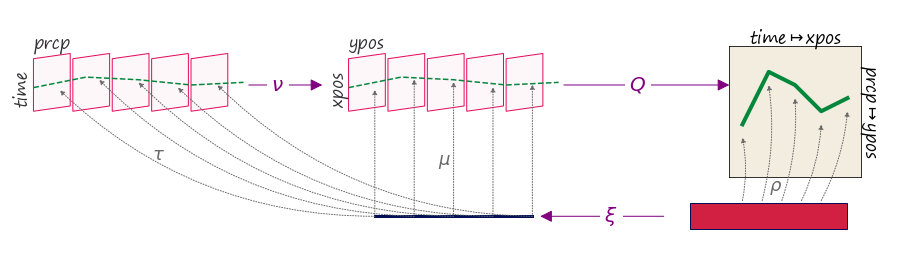
\includegraphics[width=\textwidth]{figures/math/line.png}
    \caption{The line fiber $(time,\, temp)$ is thickend with the derivative $(time^{\prime},\, temperature^{\prime}$ because that information will be necessary to figure out the tangent to the point to draw a thick line. This is because the line needs to be pushed perpendicular to the tangent of (xpos, ypos). \note{this is gonna move once this gets regenerated w/ labels} The data is converted to visual characteristics (xpos, ypos). The $\alpha$ coordinates on \gbase\ specifies the position of the line, the $\beta$ coordinate specifies thickness.}
    \label{fig:artist_line}
\end{figure}

The line plot $\vmark(xpos, \hat{n_{1}}, ypos, \hat{n_{2}})(\alpha, \beta)$ shown in fig~\ref{fig:artist_scatter} exemplifies the need for the jet discussed in section~\ref{sec:sheaf_stalk}. The line needs to know the tangent of the data to draw an envelope above and below each (xpos,ypos) such that the line appears to have a thickness. The magnitude of the thickness is 
\begin{equation}
    \lvert n \rvert = \sqrt{{n_{1}}^2 + {n_{2}}^2}
\end{equation}
such that the normal is  
\begin{equation}
    \hat{n_{1}} = \frac{n_1}{\lvert n \rvert}, \; \hat{n_{2}} = \frac{n_2}{\lvert n \rvert}
\end{equation}

which yields components of \gsection
\begin{align}
 x = xpos(\vindex(\alpha)) &+ \beta\hat(n_1)(\vindex(\alpha)) \\
 y = ypos(\vindex(\alpha)) &+ \beta\hat(n_2)(\vindex(\alpha)) 
\end{align}

where (x,y) look up the position $\vindex(\alpha)$ on the data and then apply thickness $\beta$ at that location. 

\paragraph{Q: heatmap}\mbox{} \\
\label{sec:artist_example_heatmap}
\begin{figure}[H]
    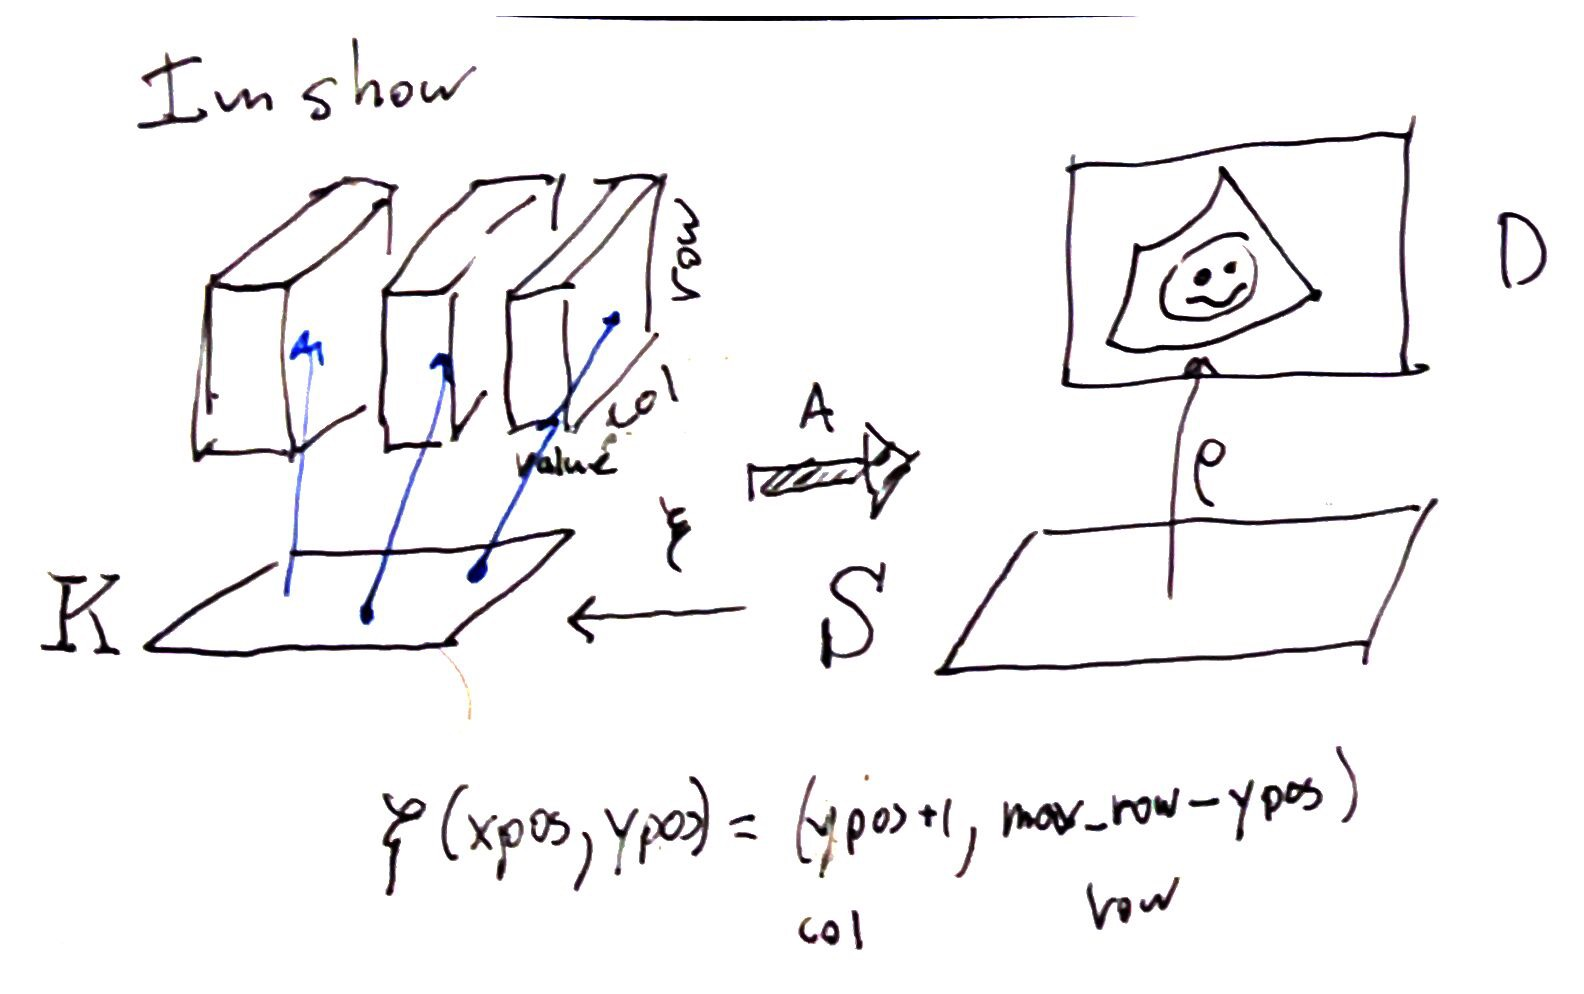
\includegraphics[width=\textwidth]{figures/math/heatmap.png}
    \caption{The only visual parameter a heatmap requires is color since \vindex\ encodes the mapping between position in data and position in graphic. }
    \label{fig:artist_heatmap}
\end{figure}

The heatmap $\vmark(color)$ in figure~\ref{fig:artist_heatmap} is a direct lookup $\vindex:\gbase\rightarrow\dbase$ such that 

\begin{align}
R &= R(\vindex(\alpha, \beta))\\
G &= G(\vindex(\alpha, \beta))\\
B &= B(\vindex(\alpha, \beta))
\end{align}
where \vindex\ may do some translating to a convention expected by \vmark\, for example reorientng the array such that the first row in the data is at the bottom of the graphic. 

\subsubsection{Equivalance class of artists $\vartist^{\prime}$}
\label{sec:artist_equivalance}
As formulated above, every artist function \vartist\ has fixed \vchannel\ and \vmark\ which  generates a distinct graphic \gsection. It is impractical to implement an artist for every single graphic; instead we implement the equivalence class of artists $\{\vartist \in \vartist^{\prime}: \vartist_{1} \equiv \vartist_{2}\}$. Equivalent artists have the same fiber bundle \vtotal\ and same assembly function \vmark\, but act on different sections \vsection. To further simplify implementation, we identify a minimal \vfiber\ associated with each $\vartist^{\prime}$ that defines what visual characteristics of the graphic must originate in the data\note{needs citation, maybe friendlys history or acquired codes of meaning}. 
\begin{figure}
    \caption{Each of these graphics is generated by a different artist \vartist which is the equivalance class of scatter plots $\vartist^{\prime}$\note{this is gonna be a whole bunch of scatter plots}}
    \label{fig:artist_equivalence}
\end{figure}
For example, a scatter plot of red circles is the output of one artist, a scatter plot of green squares the output of another, as are the rest of the graphs in figure~\ref{fig:artist_equivalance}. These two artists are equivalent since their only difference is in the literal visual encodings (color, shape). Shape and color could also be defined in \vmark\, but the position must come from the fiber $\vfiber=(xpos,ypos)$ since fundementally a scatter plot is the plotting of one position against another\cite{friendlyBriefHistoryData2008}. We also use this criteria to identify derivative types, for example the bubble chart\cite{tufteVisualDisplayQuantitative2001} is a type of scatter where by definition the glyph size is mapped from the data. 

\subsection{Making the fiber bundle computable}
\label{sec:triangulization}
\begin{figure}[H]
    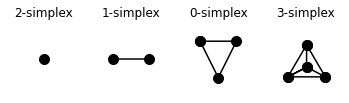
\includegraphics{figures/math/simplex.png}
    \caption{Simplices can encode the connectivity of the data, from fully disconnected (0 simplex) records to all records are connected to at least 3 others}
    \label{fig:triangle_simplex}
\end{figure}
One way of expressing the connectivity of records in a dataset is to implement \dbase\ as a simplacial complex, which is a set of simplicies such as those shown in figure~\ref{fig:triangle_simplex}. The advantage of triangulization is that it is general enough to work for more complex topology based visualization methods \cite{heineSurveyTopologybasedMethods2016} while also providing a consistent interface of vertices, edges, and faces for \vindex\ to map into. When triangulated, the simplices encode the continuity in the data

\begin{table}[H]
    \begin{center}
        \begin{tabular}{|l|l|l|}\hline
        \textbf{simplex} & \textbf{continuity} & \textbf{\dsection}   \\ \hline
        vertex  & discrete   & \dsection(\dbasepoint)                  \\ \hline
        edge    & 1D         & $\dsection(\dbasepoint,\, \alpha)$        \\ \hline
        face    & 2D         & $\dsection(\dbasepoint,\, \alpha,\, \beta)$\\ \hline
        \end{tabular}
        \caption{}
        \label{tab:triangulization}
    \end{center}
\end{table}

such that each section is bound to a simplex $\dbasepoint \in \dbase$. As shown in table~\ref{tab:triangulization}, in a 1D continuous spaces each \dsection\ lies distance $\alpha$ along edge \dbasepoint, while in a 2D continuous space each \dsection\ lies at coordinate $\alpha, \beta$ on the face \dbasepoint. This is directly analogous to indexing to express connectivity in N-D arrays, while also natively supporting graphs and trees as they are simplacial complices of nodes and edges. Path connected components are then sections where edges or faces meet. 

\begin{figure}[H]
    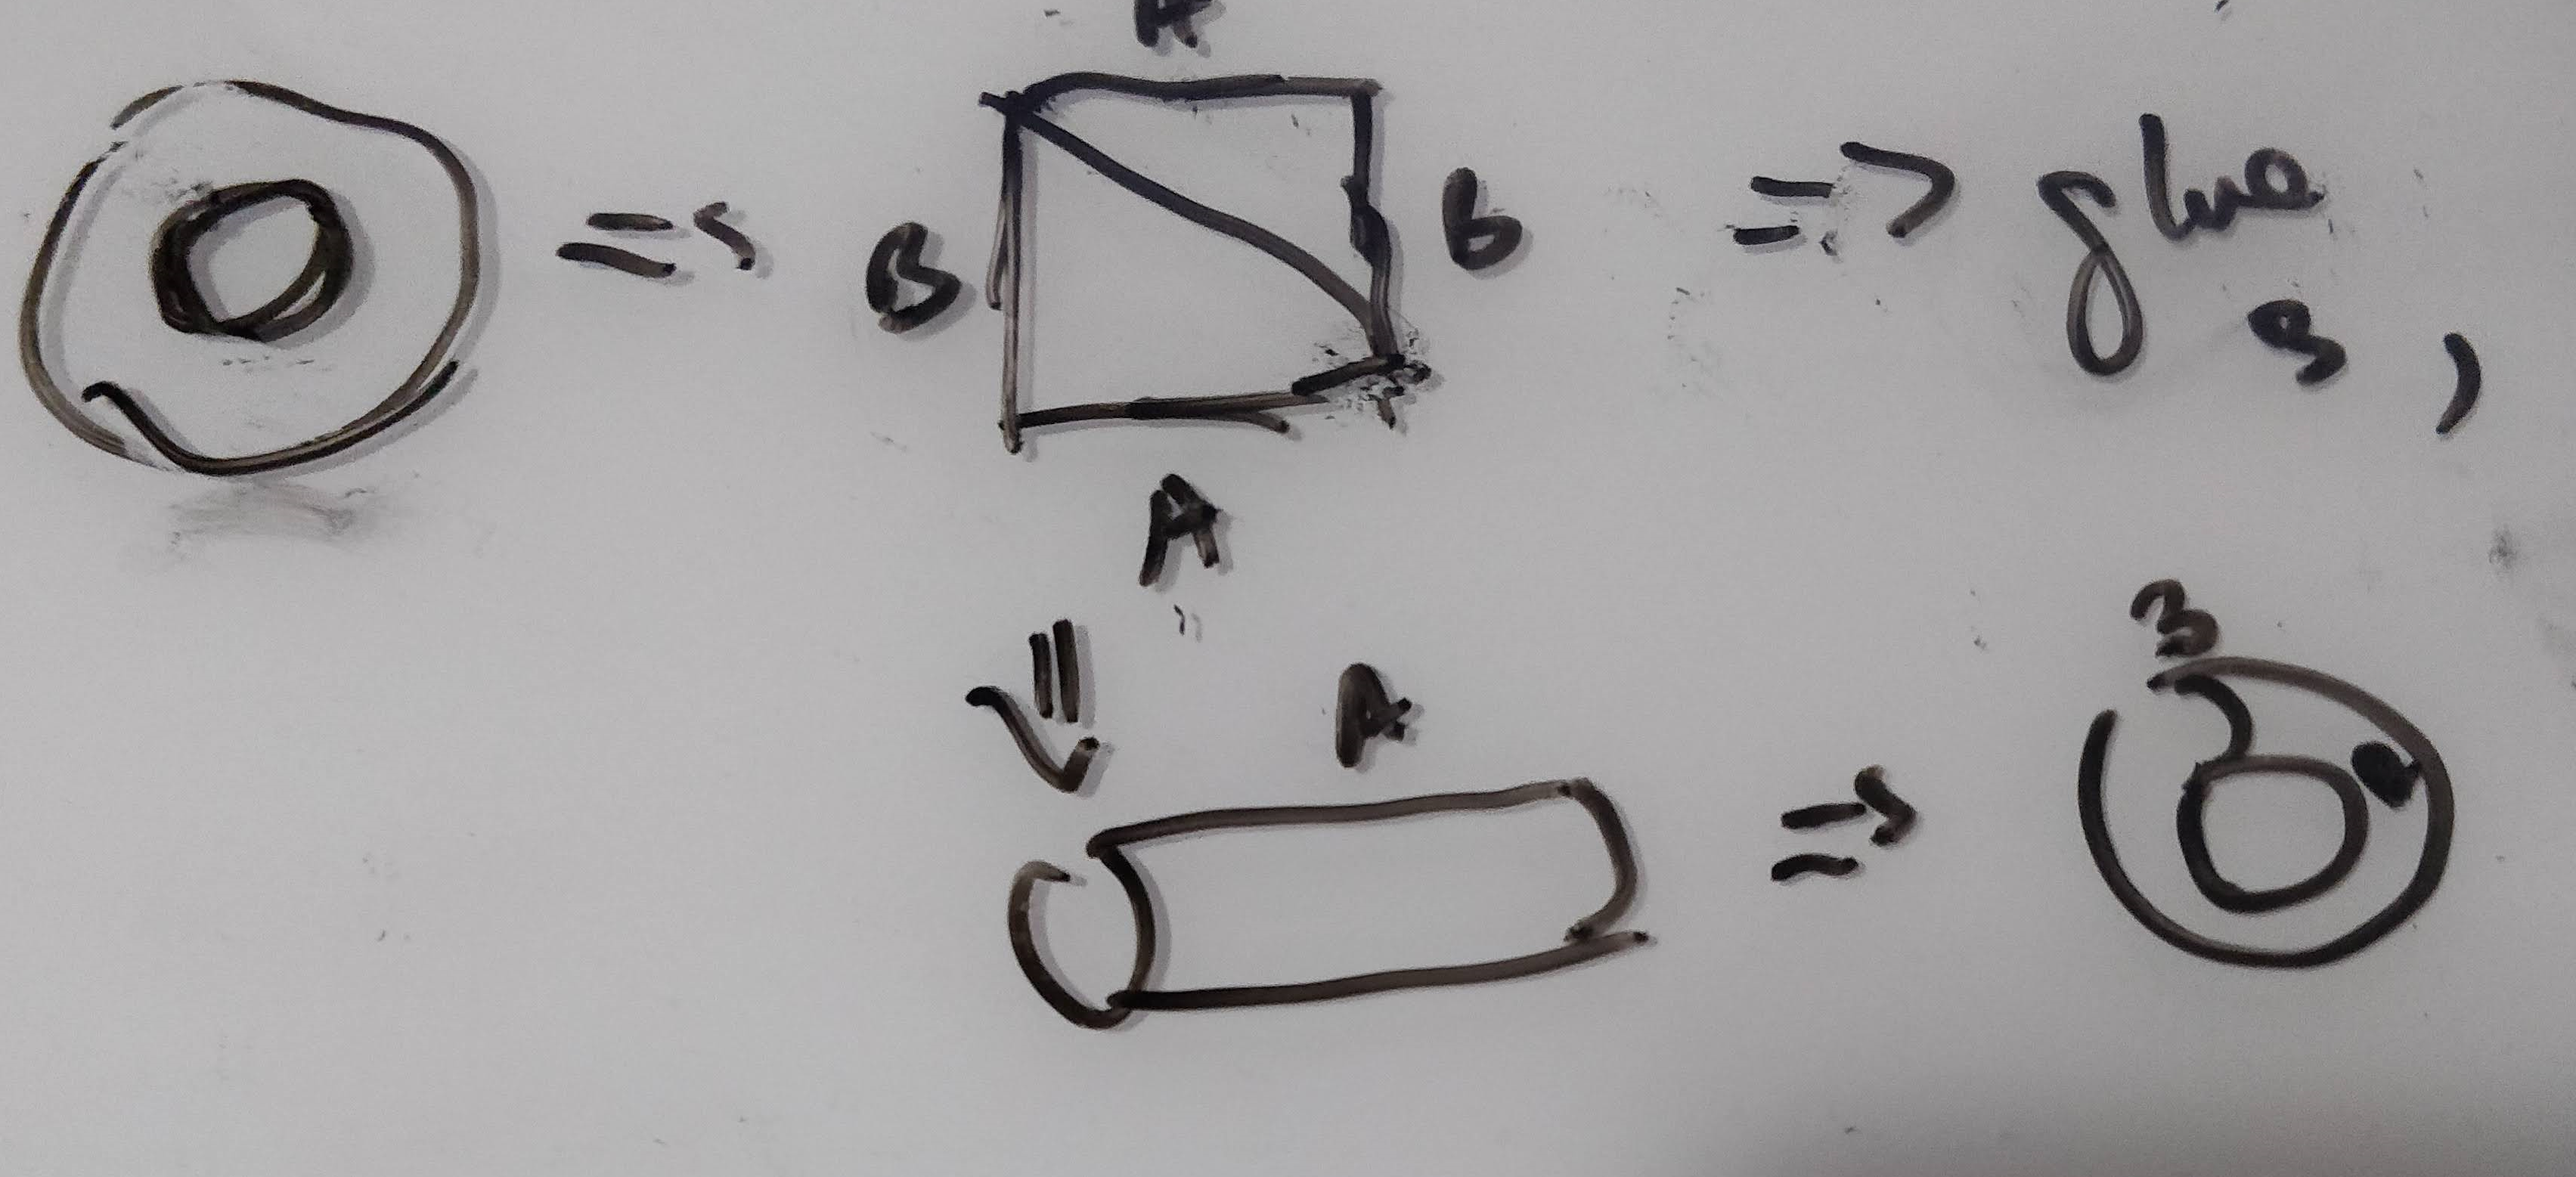
\includegraphics[width=\textwidth]{figures/math/triangle_torus.png}
    \caption{The torus \dtotal is unraveled into a simplacial complex of 2 faces \dbase. Transition functions are defined on the edges of \dbase such that surface can be glued back into the torus.
    \note{add cross sections a and b to ring and color same as edges in complex}}
    \label{fig:triangle_torus}
\end{figure}
One way of encoding the torus in figure~\ref{fig:triangle_torus} while retaining the continuity of both cross sections $a, b$ is to unravel it into a simplacial complex of two triangles with labeled edges. Transition functions $\delta$ are defined on the edges such that $a$ can be glued to $a^\prime$ and $b$ to $b^\prime$ to reconstruct the torus. This simplacial complex is then used as the base space encoding the continuity of data that lies in the torus. A constraint on the transition functions is that the monoid actions on the fibers on the edges of \dtotal\ are commutative $\monoid*\dfiber\mapsto \delta(\monoid\dfiber)= \monoid*\delta(\dfiber)$

\begin{figure}[H]
    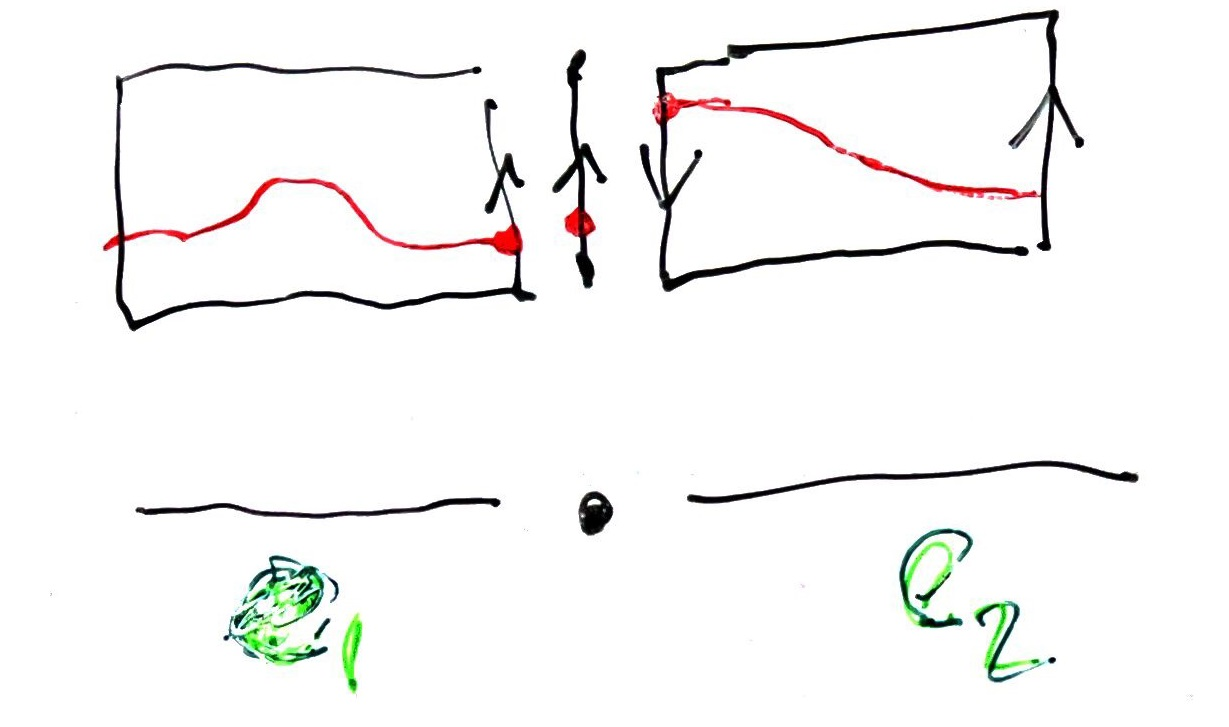
\includegraphics[width=\textwidth]{figures/math/transition_functions.png}
    \caption{Many non-trivial spaces can be made locally trivial by dividing \dtotal into locally trivial subspaces and defining transition functions between the edges on \dbase for how to glue the two subspaces such that the \dsection are continuous.}
    \label{fig:data_base_transition}
\end{figure}
Another advantages of triangulization is that it provides a way to encode non-trivial structures such as the mobius strip\cite{MobiusStripNLab}. As shown in figure ~\ref{fig:data_base_transition}, one way of making the mobius strip trivial is to seperate it into two spaces $\dtotal_1$ and $\dtotal_2$ and then define transition functions that specify that the edges of $\dtotal_1$ need to be reversed to line up with $\dtotal_2$ such that the sections along the edges meet. As with the torus, the transition functions must preserve monoid commutativity. 


\end{document}